\lstset{language=R,
    basicstyle=\small\ttfamily,
    stringstyle=\color{gray},
    otherkeywords={0,1,2,3,4,5,6,7,8,9},
    morekeywords={TRUE,FALSE},
    deletekeywords={data,frame,length,as,character},
    keywordstyle=\color{blue},
    commentstyle=\color{gray},
    numbers=left,
    stepnumber=1
}

\chapter{Data Understanding Preliminare}
\label{ch:undst}

La fase che verrà descritta in seguito è fra le più delicate di tutto il processo di \textit{data mining}. Da essa dipende la buona riuscita o meno dell'intera attività di estrazione d'informazioni. Come appare quindi naturale, è stata dedicata a essa una particolare attenzione.

    \section{Introduzione al Data Understanding}

        Perché occorre spendere del tempo per perpetrare un'estesa fase di \textit{data understanding}? \\

        Banalmente, l'obiettivo principale che ci si prefigge è quello di ottenere una chiara visione d'insieme sui dati che si hanno a disposizione. In questo modo, si sarà in grado di prendere decisioni oculate per quanto riguarda il da farsi nei successivi passi di questa analisi. Si prenda ad esempio l'attività di \textit{preprocessing}: sintetizzando al massimo, possiamo dire che si tratta di lavorare dei dati grezzi al fine di renderli adatti a essere processati da certi algoritmi. L'ovvia implicazione è che occorre avere ben chiaro in anticipo quali algoritmi sarà opportuno lanciare, fatto che a sua volta implica la necessità di conoscere quali informazioni si intende estrarre dai dati grezzi a disposizione. \\

        Questo aspetto rende necessario far precedere a quello che è, usando una metafora nell'ambito meccanico, l'attività di sgrossatura dei dati grezzi una fase di \textit{data understanding}. \\

        In questa sezione, quindi, si punterà a capire a fondo la natura dei dati al fine d'intuire che cosa sia possibile trarne.

        \subsection{Metodi e Strumenti}

            L'attività di \textit{data understanding} può essere svolta in molti modi, non essendoci delle regole fisse che la disciplinano rigidamente. Si può azzardare che le risorse più importanti alle quali si può attingere in questo ambito sono, piuttosto romanticamente, l'intuito e la fantasia dei \textit{data scientist} coinvolti nel progetto. Fuori di metafora, è chiaro che non esistano procedure che indichino univocamente le informazioni che è possibile ricavare su un dato insieme di dati. Perciò, quello che occorre fare è sfruttare dei metodi che riassumano i dati per poterli apprezzare nel loro insieme. \\

            Gli strumenti più adatti per poter ottenere una visione d'insieme sull'intera mole di dati sono, senza ombra di dubbio, le varie \textit{tecniche di visualizzazione} esistenti. Il loro utilizzo è stato permesso da software quali \textbf{R} e \textbf{Weka}, oltre che da più comuni \textit{spreadsheet} forniti da suite di programmi da ufficio. \footnote{Per un maggior dettaglio, si consulti il capitolo riguardo alla \textit{technology stack} impiegata per la realizzazione di questo progetto.}

    \section{Data Set: Produttività degli Studenti}

        Senza ombra di dubbio questa porzione di dati rappresenta la più significativa dell'intero lotto a disposizione per questa analisi. \\

        Si è quindi optato per utilizzare il software \textbf{R}, in quanto consente d'impiegare efficientemente un gran numero di approfondite tecniche di visualizzazione. Tuttavia, la potenza e la flessibilità offerte da questo tipo di strumento si pagano con la necessita di dedicare un minimo di attenzione all'importazione del data set in quell'ambiente di lavoro. \\

        In senso pratico, questo si traduce nel lanciare del codice analogo \footnotesize{--- non identico: sono stati accorciati i percorsi ---}\normalsize\ a quanto mostrato di seguito prima di poter effettuare qualunque altra operazione. \\

        \begin{lstlisting}
# set the repo root path before importing data!!!
setwd("C:/a/path/to/somewhere")
students <- read.csv("raw/prod_stud.csv")

# gather some info about the imported data set
str(students)

# ADJUST DATA ATTRIBUTES
# convert "coorte" to nominal by making it a factor
students[, c(1)] <- sapply(students[, c(1)], factor)

# ok, let's take a look at it now
str(students)
summary(students)
        \end{lstlisting}

        In ogni caso, dato l’elevato numero degli attributi del data set, è stato necessario prendere delle decisioni relative a cosa visualizzare – e con quale tecnica. Le scelte sono state ovviamente compiute su base intuitiva, a seguito di un’analisi sommaria delle caratteristiche del data set. \\

        È stato quindi deciso di effettuare una ricerca visiva di correlazioni fra valori di attributi relativi a:

        \begin{itemize}
            \item prestazioni generali durante tutto il periodo esaminato
            \item prestazioni nei singoli esami
            \item risultati di gruppi di esami
        \end{itemize}

        \subsection{Prestazioni Generali degli Studenti}

            Lo script \textbf{R} che segue disegna dei grafci di dispersione su coppie di attributi relativi alle prestazioni generali degli studenti. Lo scopo è quello di individuare visivamente delle correlazioni significative fra questi attributi.\\

            \begin{lstlisting}
colors <- c("blue","red", "green", "orange")
coorte_labels <- students[,1]
coorte_colors <- colors[as.numeric(coorte_labels)]
library(seriation)

# general attributes
students_subset1 <- students[,-c(1, 6 : 45)]
pairs(students_subset1, col = coorte_colors,lower.panel = 	NULL,cex.labelsiris=2, pch=19, cex = 1.2)
par(xpd = TRUE)
legend(x = 0.05, y = 0.4, cex = 1,legend = 	as.character(levels(coorte_labels)),fill = unique(coorte_colors))
par(xpd = NA)
            \end{lstlisting}

            \begin{figure}
                \caption{grafici di dispersione riguardanti attributi generali del data set degli studenti}
                \label{fig1}
            	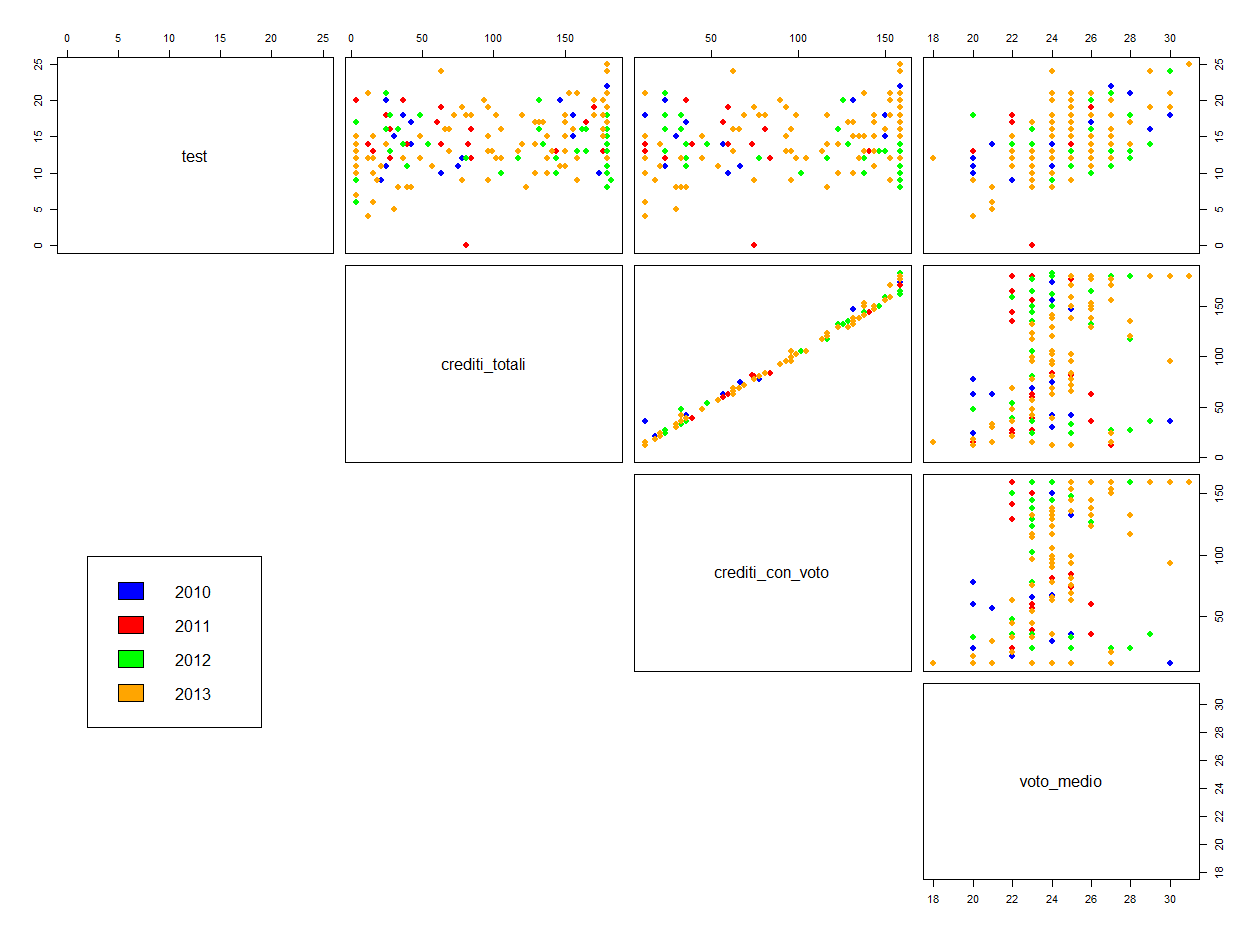
\includegraphics[scale=0.33]{img/scatter_plot_1_gen.png}
            \end{figure}

            Come si può vedere sul grafico generato dallo script --- mostrato in Figura \ref{fig1} --- esistono varie correlazioni fra gli attributi considerati. Nel merito, la relazione fra le quantità \textit{crediti totali} e \textit{crediti con voto} è tanto palese quanto banale: il primo ammontare contiene il secondo, e la loro differenza è minima. Appare invece più interessante quello che accade fra altre coppie di attributi:

            \begin{itemize}
                \item punteggio del test di ingresso e valore atteso del voto
                \item quantità di crediti ottenuti e valore atteso del voto
            \end{itemize}

            Si ritiene quindi opportuno realizzare dei grafici che abbiano un maggior livello di dettaglio su questi aspetti. \\

            \begin{figure}
                \centering
                \caption{grafico di dispersione sugli attributi "voto medio" e "test di ingresso"}
                \label{fig2}
            	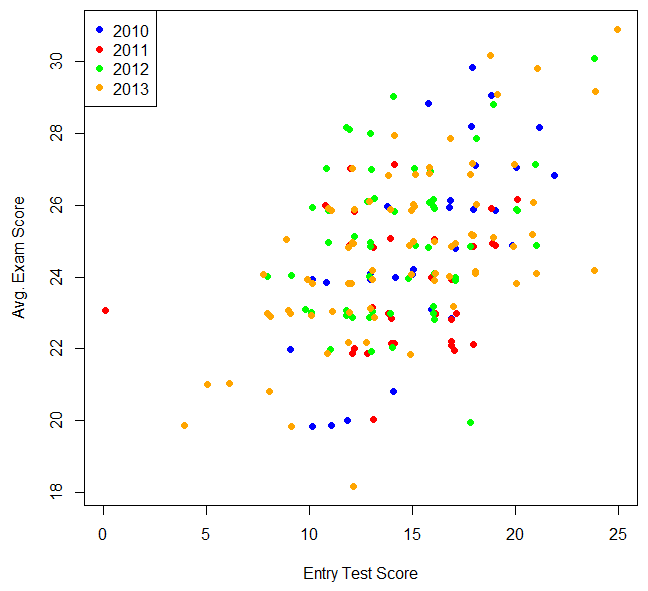
\includegraphics[scale=0.80]{img/scatter_plot_2.png}
            \end{figure}

            \begin{figure}
                \centering
                \caption{grafico di dispersione sugli attributi "voto medio" e "C.F.U. ottenuti"}
                \label{fig3}
            	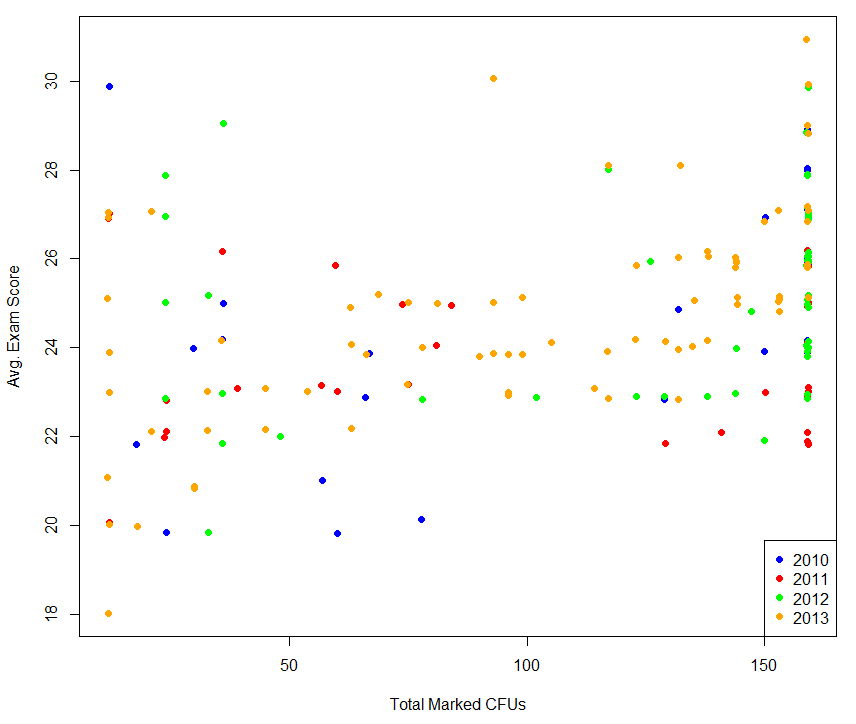
\includegraphics[scale=0.62]{img/scatter_plot_3.png}
            \end{figure}

            Come risulta dalla Figura \ref{fig2}, si potrebbe speculare che esista una correlazione lineare fra i due attributi: gli studenti che conseguono un punteggio alto nel test di ingresso sono più propensi ad ottenere voti alti negli esami. \\

            Per quanto riguarda invece la Figura \ref{fig3}, fra gli studenti che hanno conseguiti tutti i crediti si può notare una consistente densità nella fascia che va circa dal ventidue al ventinove. Si può anche notare una assenza di voti medi inferiori al 22 fra coloro che hanno conseguito più di 100 CFU. Un altro aspetto che potrebbe rivelarsi interessante è che, fra la coorte di studenti del 2013, vari studenti hanno conseguito un solo esame con un voto superiore al 20. \\

            Viste le possibili informazioni che sembra possibile estrarre, si è deciso d'insistere sull’analisi visiva degli attributi \textit{voto medio} e \textit{numero totale di crediti}. Sono stati quindi realizzati dei diagrammi a scatola e baffi con il seguente script \textbf{R}: 

            \begin{lstlisting}
boxplot(students[,4]~students[,1],data = students,xlab="Total Marked CFU",col=colors)
boxplot(students[,5]~students[,1],data = students,xlab="Avg. Exam Score",col=colors)
            \end{lstlisting}

            \begin{figure}
                \centering
                \caption{diagramma a scatole e baffi relativo all'attributo "numero totale di crediti"}
                \label{boxplot1}
            	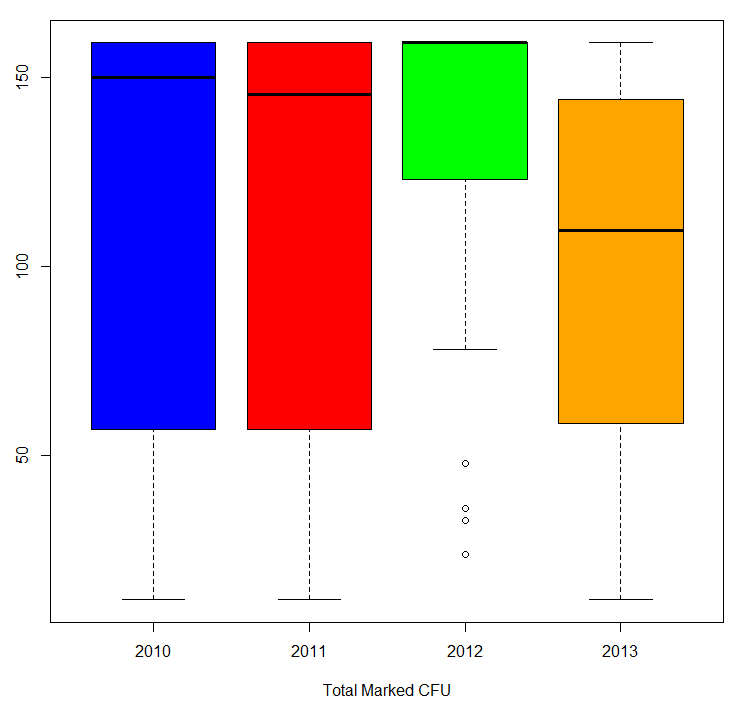
\includegraphics[scale=0.55]{img/box_plot_1.png}
            \end{figure}

            \begin{figure}
                \centering
                \caption{diagramma a scatole e baffi relativo all'attributo "voto medio"}
                \label{boxplot2}
            	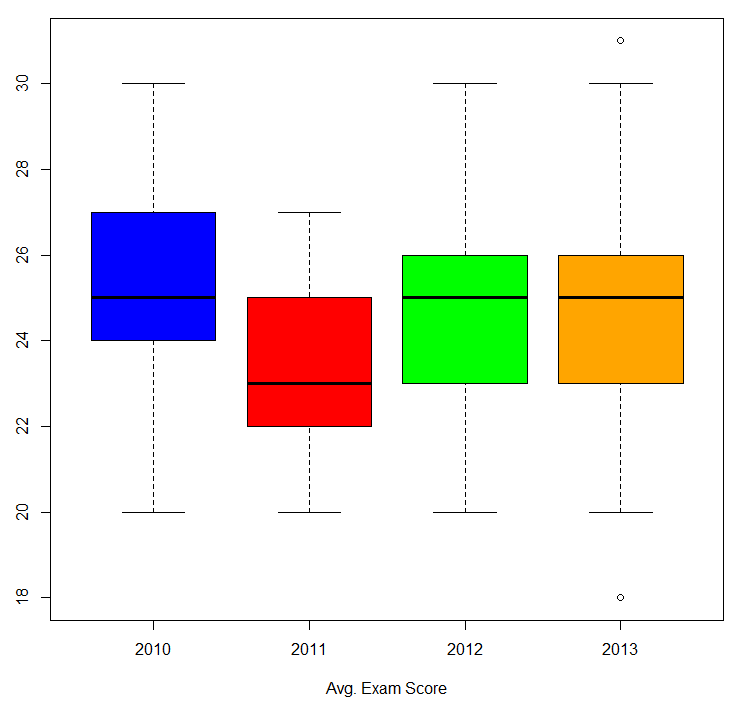
\includegraphics[scale=0.70]{img/box_plot_2.png}
            \end{figure}

            Riguardo al diagramma in Figura \ref{boxplot1}, si noti come gli immatricolati nelle annate 2010 e 2011 hanno prestazioni molto simili sul fronte dei crediti conseguiti. La coorte 2012 risulta la migliore, avendo addirittura per mediana il massimo ammontare di crediti ottenibili\footnote{non si ignorino però le istanze considerate \textit{outliers} dall’algoritmo!}, mentre gli studenti immatricolati nel 2013 sono stati i meno performanti. Nel caso invece del voto medio, rappresentato in Figura \ref{boxplot2}, si evidenzia solo un leggero peggioramento negli immatricolati nel 2011 rispetti alle altre coorti di studenti. Sono degni di attenzione anche i due \textit{outliers} nella coorte 2013.

        \subsection{Prestazioni degli Studenti su Gruppi di Esami}

            Una scelta significativa nell’ambito di questa fase è stata la suddivisione degli esami in vari gruppi. Si è cercato di raggruppare intuitivamente degli esami i cui risultati potrebbero essere correlati in qualche modo. L’ovvio rischio che si è scelto di correre è quello di non notare correlazioni che esistono, ma che non sono intuitive. \\

            La suddivisione più sensata è sembrata essere la seguente:

            \begin{itemize}
                \item esami del primo anno
                \item esami su argomenti principalmente informatici
                \item esami su argomenti principalmente matematici
            \end{itemize}

            \subsubsection{Esami del primo anno}

                Il seguente script \textbf{R} ha generato i grafici di dispersione, le matrici di correlazione e di deviazione standard utilizzate per l’analisi visiva del gruppo di esami del primo anno. Per gli altri gruppi di esami, gli script sono stati molto simili.

                \begin{lstlisting}
# general first year exams performances
students_subset2 <- students[,-c(1 : 5, 7, 9, 11, 13, 15 : 45)]
pairs(students_subset2, col = coorte_colors,lower.panel = NULL,cex.labelsiris=2, 	pch=19, cex = 1.2)
par(xpd = TRUE)
legend(x = 0.05, y = 0.4, cex = 1,legend = as.character(levels(coorte_labels)),fill 	= unique(coorte_colors))
par(xpd = NA)

students_scaled <- scale(students_subset2)
pimage(students_scaled,ylab="Students",main="Standard Deviations from Mean Mark")

matrix <- as.matrix(students_scaled)
cm <- cor(t(matrix), method="pearson")
pimage(cm,main="Correlation Matrix considering 1st Year exams", xlab="Students", 	ylab="Students",zlim = c(-1,1),col = bluered(50))
                \end{lstlisting}

                \begin{figure}
                    \centering
                    \caption{grafici di dispersione riguardanti gli attributi relativi agli esami del primo anno}
                    \label{esami1anno_sp}
                	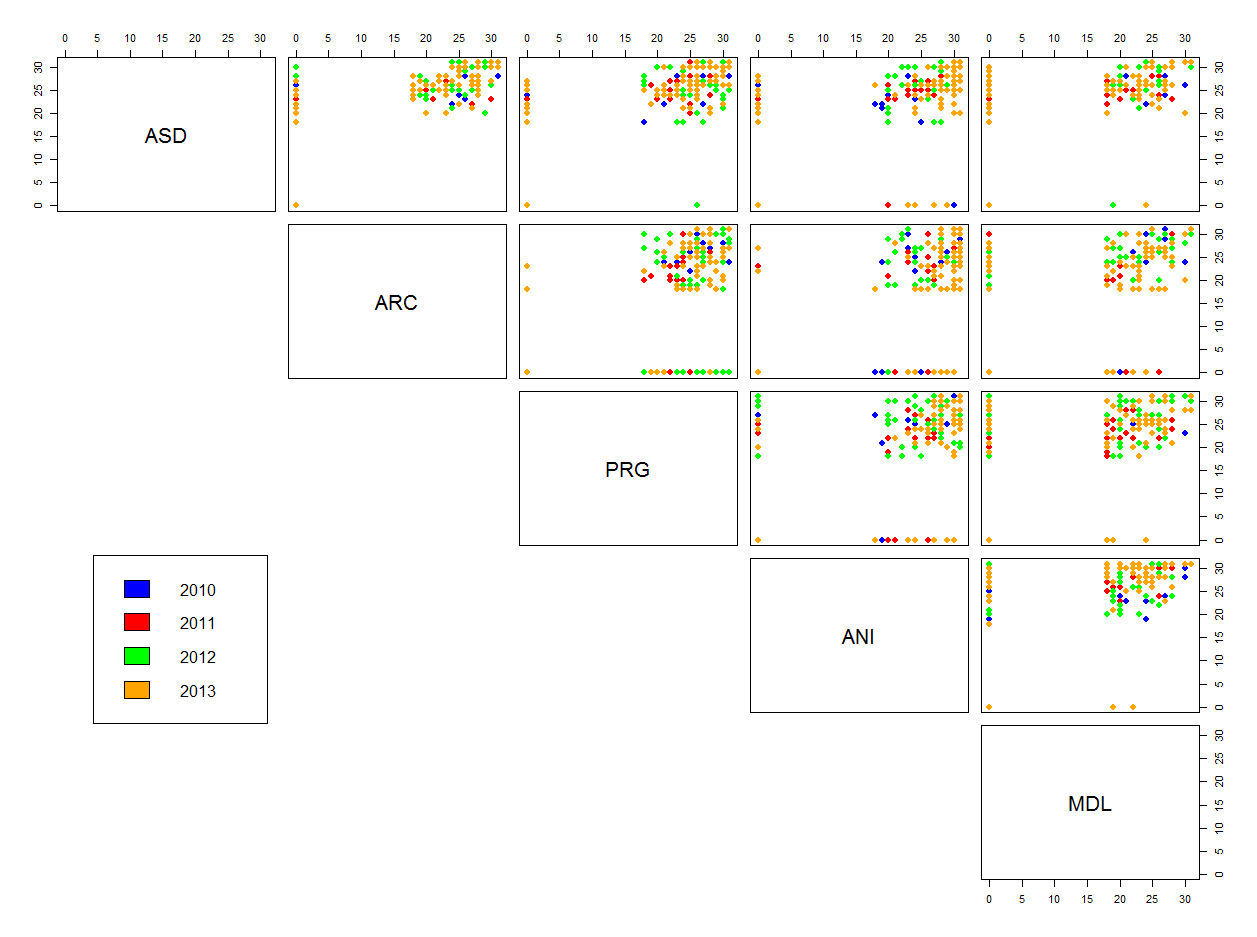
\includegraphics[scale=0.34]{img/scatter_plot_4_gen.png}
                \end{figure}

                Dall’analisi visiva del grafico di dispersione in Figura \ref{esami1anno_sp} non si è stati in grado di concludere molto di concreto. Eppure si ritiene possibile che qualche informazione interessante si possa nascondere dentro l’insieme di dati degli esami del primo anno; occorre scendere nel dettaglio. A questo proposito, sono state realizzate le matrici delle Figure \ref{esami1anno_corr} e \ref{esami1anno_stddev}. \\

                \begin{figure}
                    \centering
                    \caption{matrice di correlazione fra le istanze degli studenti, considerante i risultati degli esami del primo anno}
                    \label{esami1anno_corr}
                	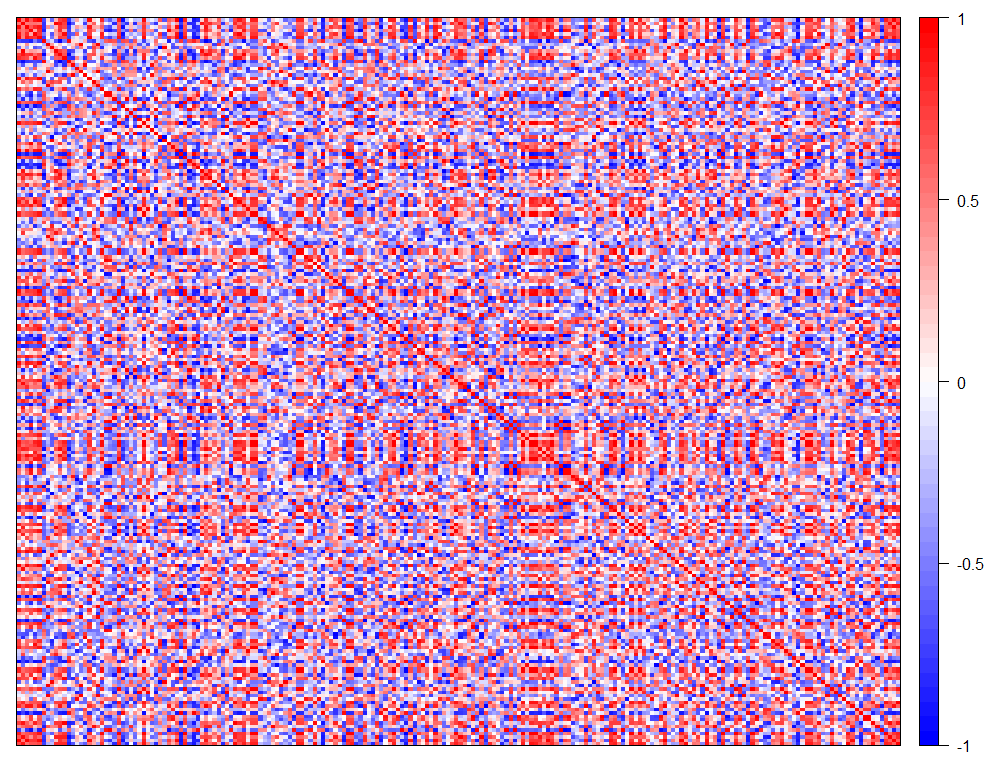
\includegraphics[scale=0.35]{img/corr_matrix_1.png}
                \end{figure}

                \begin{figure}
                    \centering
                    \caption{matrice dello scarto quadratico medio dei risultati degli esami da sostenere il primo anno}
                    \label{esami1anno_stddev}
                	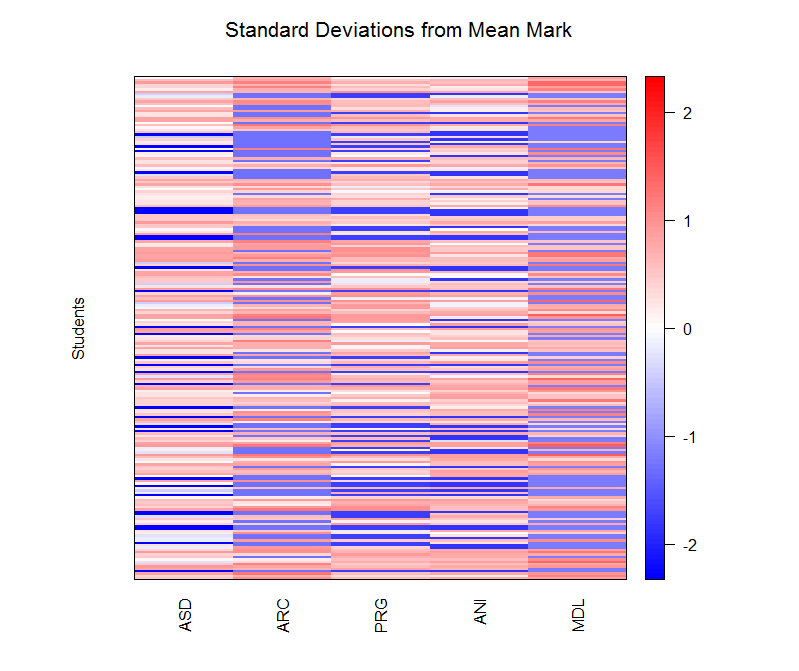
\includegraphics[scale=0.60]{img/std_dev_matrix_1.png}
                \end{figure}

                Per quanto riguarda invece quanto mostrato in Figura \ref{esami1anno_corr}, come misura di correlazione è stata scelta la \textit{correlazione di Pearson}, ricercando quindi relazioni monotone --- vengono considerati simili studenti che hanno un andamento simile su un gruppo sufficientemente grande di esami, senza contare eventuali \textit{offset} fra le valutazioni. Si nota un accenno di trama in due punti, sintomo di similarità fra due fasce di studenti. Quesrto può far pensare che potrebbe essere possibile individuarle con algoritmi di \textit{clustering}. \\

                Osservando invece la Figura \ref{esami1anno_stddev}, si può evidenziare che i colori più tiepidi della deviazione standard per gli esami di \textit{Matematica Discreta e Logica} e \textit{Architetture degli Elaboratori} stanno ad indicare una minore tendenza a discostarsi dal voto medio. Perché studenti di vari anni tendono a convergere verso lo stesso voto in quei due esami? Per rispondere a questa domanda, si veda in Figura \ref{1annosommario} un sommario dell'attributo \textit{data}. \\

                \begin{figure}
                    \centering
                    \caption{sommario dell'attributo "data" relativo agli esami del primo anno}
                    \label{1annosommario}
                	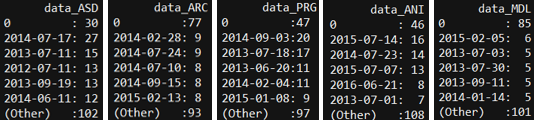
\includegraphics[scale=0.70]{img/sommario_1_anno.png}
                \end{figure}

                Gli esami che non sono stati superati dal maggior numero di istanze dell’intero data set --- e che quindi hanno creato maggiore difficoltà agli studenti --- sono Matematica Discreta e Logica e Architetture degli Elaboratori. Si è inoltre notato nella matrice della derivazione standard mostrata in Figura \ref{esami1anno_stddev} che quei due esami presentano una differenza rispetto agli altri. Vale la pena di indagare oltre. \\

                \begin{figure}
                    \centering
                    \caption{grafico di dispersione fra gli attributi "voto ottenuto a Matematica Discreta e Logica" e "C.F.U. ottenuti nel periodo in esame"}
                    \label{mdl}
                	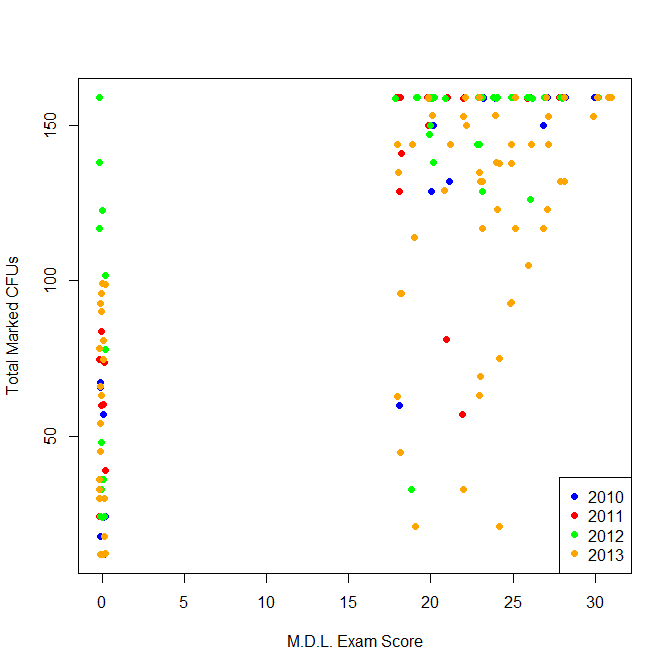
\includegraphics[scale=0.60]{img/scatter_plot_5.png}
                \end{figure}

                \begin{figure}
                    \centering
                    \caption{grafico di dispersione fra gli attributi "voto" e "data di superamento" relativi all'esame di Matematica Discreta e Logica}
                    \label{mdl_2}
                	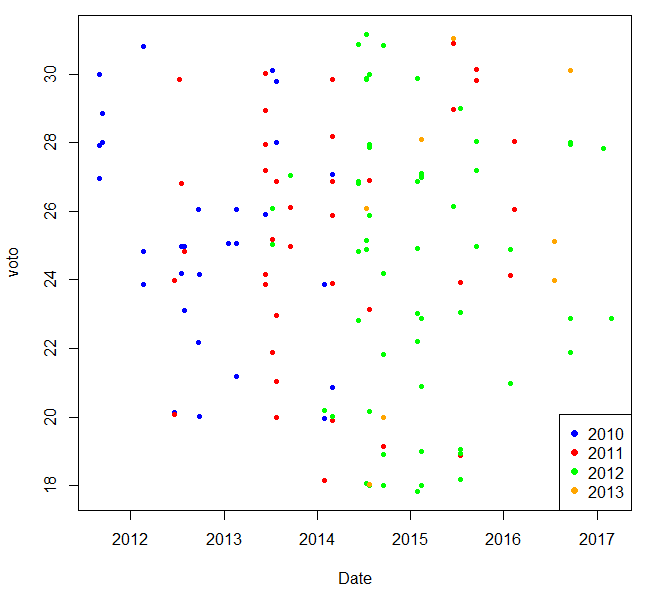
\includegraphics[scale=0.6]{img/scatter_plot_9.png}
                \end{figure}

                \begin{figure}
                    \centering
                    \caption{grafico di dispersione fra gli attributi "voto ottenuto a Architetture degli Elaboratori" e "C.F.U. ottenuti nel periodo in esame"}
                    \label{ade}
                	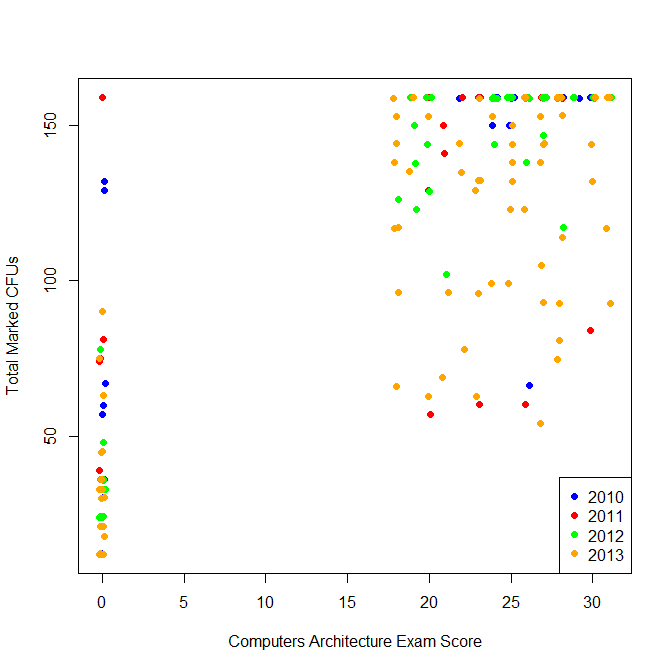
\includegraphics[scale=0.6]{img/scatter_plot_6.png}
                \end{figure}

                Si veda il grafico di dispersione specifico per Matematica Discreta e Logica in Figura \ref{mdl}: si riesce a notare una blanda tendenza dei Credti Formativi Unitari ottenuti in totale dallo studente ad aumentare proporzionalmente al voto ottenuto. C’è inoltre una chiara indicazione che molti studenti –-- con quelli della coorte 2012 a estremizzare questa caratteristica –-- hanno ottenuto comunque molti C.F.U. senza superare questo esame. Inoltre, incrociando il voto conseguito e la data in cui l’esame è stato superato (si veda la Figura \ref{mdl_2}), si riescono a notare due aspetti:

                \begin{itemize}
                    \item chi ha dato l’esame al primo appello del suo anno, ha conseguito un voto alto (si vedano ad esempio gli studenti dell’annata 2010)
                    \item la maggioranza degli studenti ha superato Matematica Discreta e Logica qualche anno dopo il suo anno di immatricolazione (comportamento estremizzato dagli studenti di coorte 2012)
                \end{itemize}

                Nel caso di Architetture degli Elaboratori, della quale possiamo vedere un grafico di dispersione dettagliato in Figura \ref{ade}, le tendenze evidenziate prima sono mitigate. Rimane comunque importante la quantità di studenti che hanno conseguito molti crediti senza superare l’esame: si potrebbe speculare che l’ignorare certi esami sia una pratica comune nel pool di studenti descritti dal data set.

            \subsubsection{Esami su argomenti informatici}

                \begin{figure}
                    \centering
                    \caption{grafici di dispersione relativi agli esami a contenuto prevalentemente informatico}
                    \label{esami_inf}
                	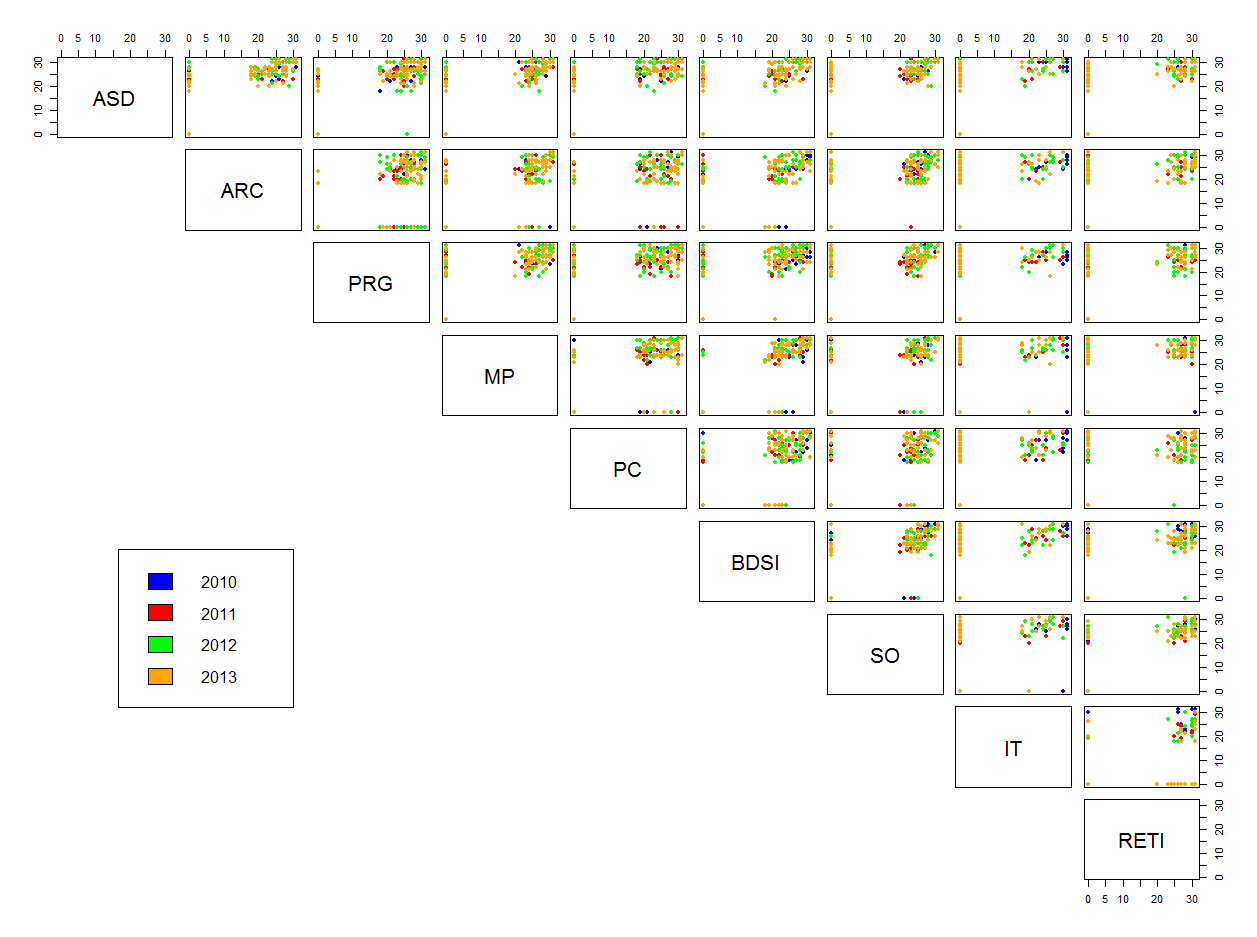
\includegraphics[scale=0.32]{img/scatter_plot_7_gen.png}
                \end{figure}

                \begin{figure}
                    \centering
                    \caption{matrice di correlazione fra gli studenti, considerante i risultati ottenuti negli esami di informatica}
                    \label{esami_inf_corr}
                	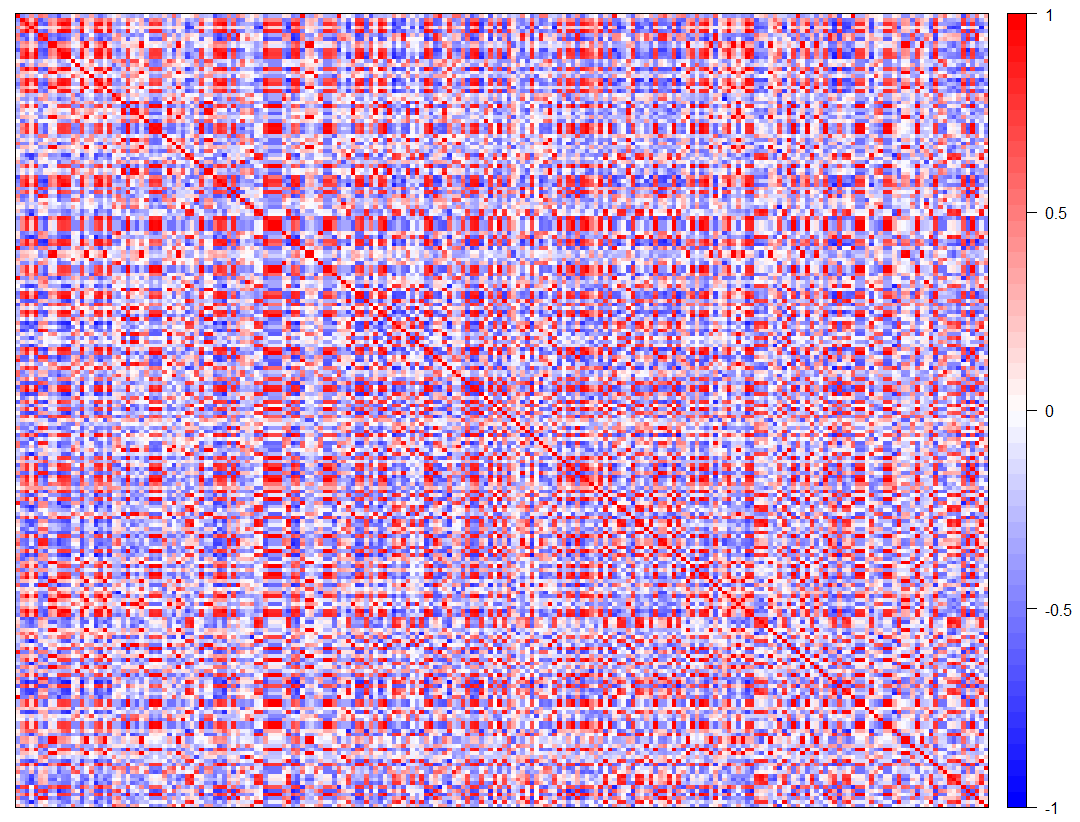
\includegraphics[scale=0.32]{img/corr_matrix_2.png}
                \end{figure}

                \begin{figure}
                    \centering
                    \caption{matrice dello scarto quadratico medio dei risultati degli esami ad argomento informatico}
                    \label{esami_inf_stddev}
                	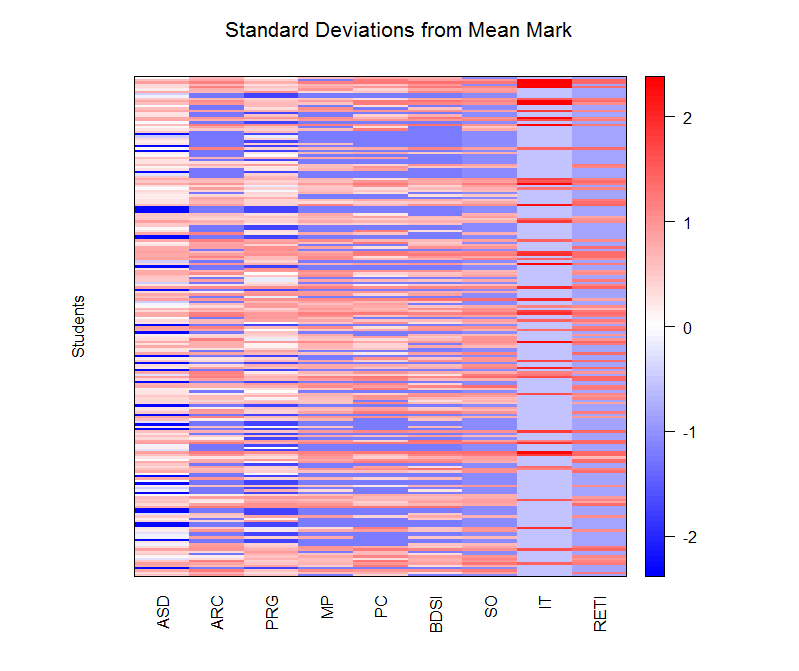
\includegraphics[scale=0.6]{img/std_dev_matrix_2.png}
                \end{figure}

                \begin{figure}
                    \centering
                    \caption{sommario dell'attributo "voto" relativo all'esame di Informatica Teorica}
                    \label{it}
                	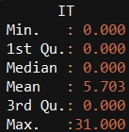
\includegraphics[scale=0.75]{img/it.png}
                \end{figure}

                Riguardo agli esami a contenuto prevalentemente informartico, sono state effettuate analoghe analisi visive. Poco è stato notato dal grafico di dispersione in Figura \ref{esami_inf} e dalla matrice di correlazione in Figura \ref{esami_inf_corr}. Invece, dalla matrice della deviazione standard in Figura \ref{esami_inf_stddev} è stato possibile trarre una interessante deduzione: con l’avvicinarsi agli esami del terzo anno –-- eccezione fatta per Architetture degli Elaboratori –-- si nota che il voto conseguito da ogni studente tende a discostarsi sempre meno dalla media. Nel particolare di Informatica Teorica mostrato in Figura \ref{it}, i pochi studenti che lo superano risultano ampiamente sopra la media. \\

                In ogni caso, non appare interessante proseguire sul'analisi con tecniche di \textit{data mining} su questa suddivisione.

            \subsubsection{Esami su argomenti matematici}

                \begin{figure}
                    \centering
                    \caption{grafici di dispersione relativi agli esami ad argomento prevalentemente matematico}
                    \label{esami_mat}
                	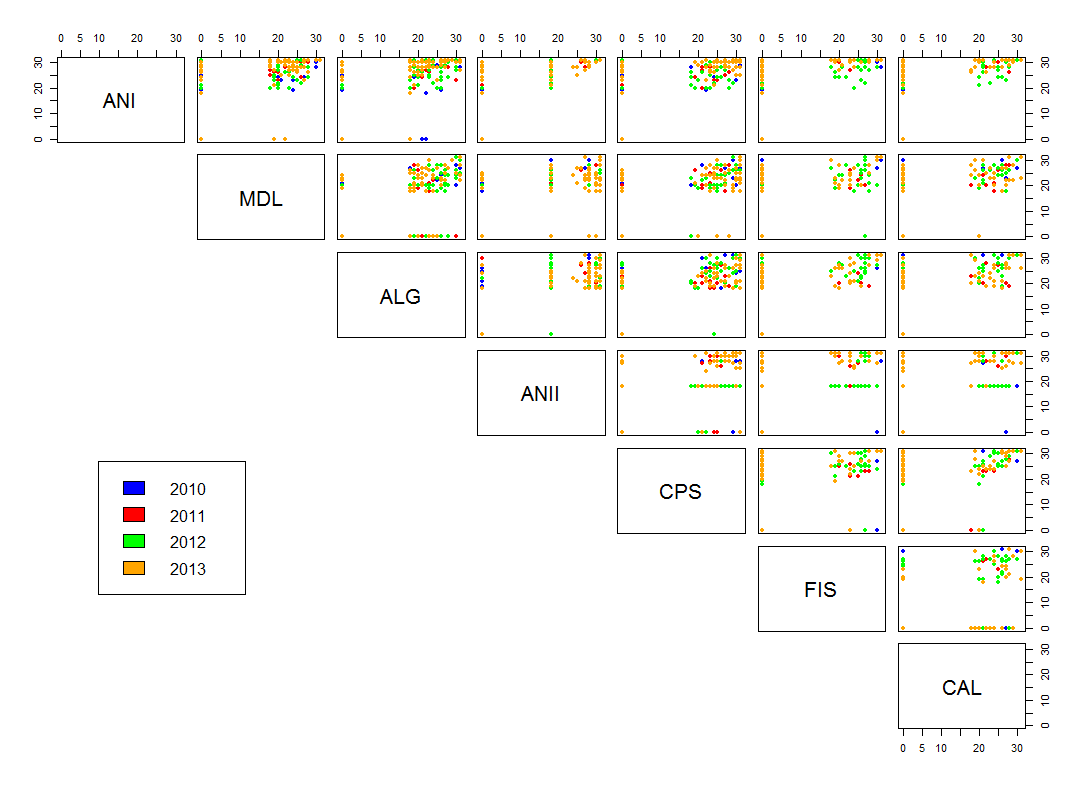
\includegraphics[scale=0.38]{img/scatter_plot_8_gen.png}
                \end{figure}

                \begin{figure}
                    \centering
                    \caption{matrice di correlazione fra gli studenti, considerante i risultati degli esami di matematica}
                    \label{esami_mat_corr}
                	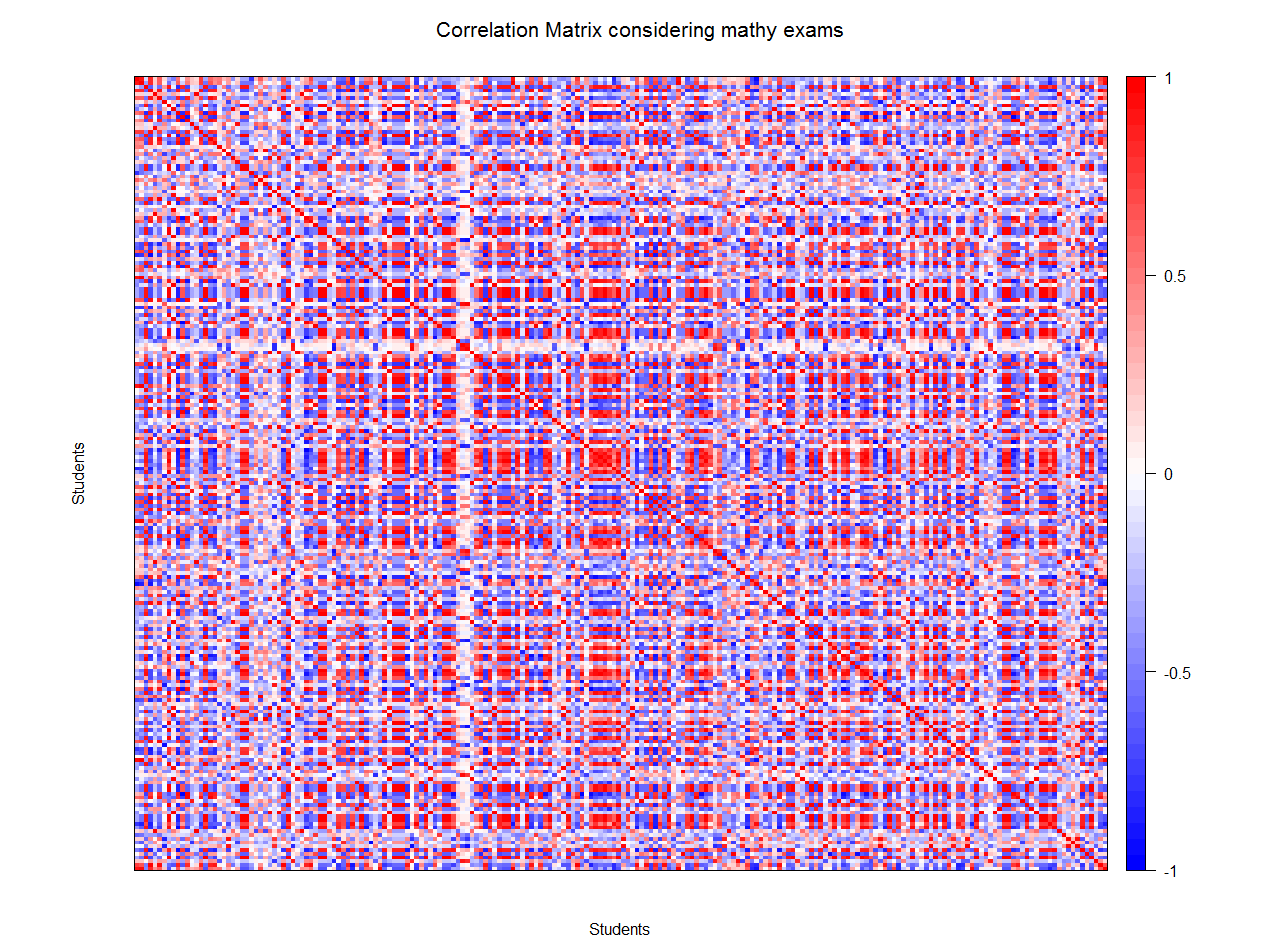
\includegraphics[scale=0.32]{img/corr_matrix_3.png}
                \end{figure}

                \begin{figure}
                    \centering
                    \caption{matrice dello scarto quadratico medio dei risultati degli esami a contenuto matematico}
                    \label{esami_mat_stddev}
                	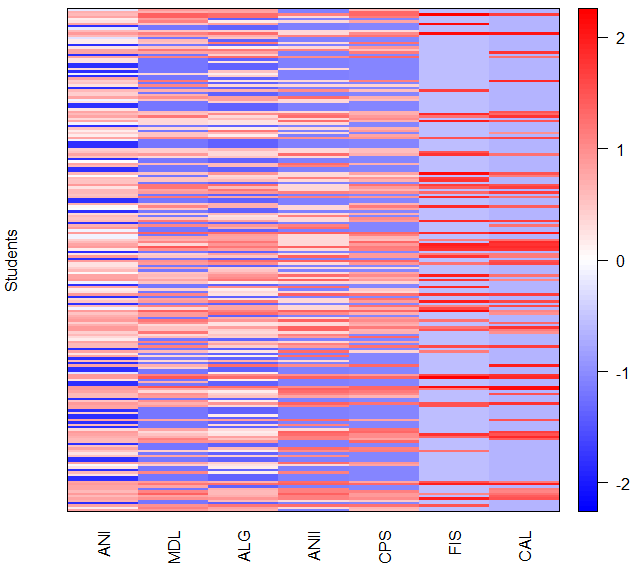
\includegraphics[scale=0.6]{img/std_dev_matrix_3.png}
                \end{figure}

                Riguardo a questa partizione degli esami, di cui si può vedere un grafico di dispersione generale in Figura \ref{esami_mat}, un aspetto che balza immediatamente alla vista è l’enorme quantità di studenti che ha conseguito 18 ad Analisi 2. Date le modalità di esame previste per il corso\footnote{se le prove intermedie scritte risultano sufficienti, si può accettare un voto di 18 senza sostenere la prova orale}, questa non è affatto un'anomalia, pertanto non appare interessante; inoltre, potrebbe addirittura risultare distorcente rispetto ad una ipotetica \textit{cluster analysys}, perciò occorrerebbe considerarla preventivamente.\\

                Sulla matrice di correlazione in Figura \ref{esami_mat_corr}, si notano due aspetti interessanti: una fascia di studenti con correlazione nulla e una «casella» di forti correlazioni all’incirca nel centro della matrice. Dei due, il primo è sicuramente il più inusuale. Quale aspetto reale potrebbe generare una osservazione come questa?\\

                Riguardo alla matrice della deviazione standard in Figura \ref{esami_mat_stddev}, si possono notare le stesse caratteristiche evidenziate per quanto riguarda gli esami a tema principalmente informatico. In questo caso, il ruolo del cattivo non lo interpreta più Informatica Teorica ma è condiviso da Fisica Generale e Calcolo Numerico\footnote{Calcolo Numerico tratta argomenti che trascendono i confini fra l’informatica e la matematica. Si è scelto d'inserirlo in questa partizione, ma è stata una decisione puramente arbitraria.}.\\

                Analogamente alla suddivisione precedente, anche per questa partizione di esami non appare interessante proseguire l'analisi con tecniche di \textit{data mining}.

        \subsection{Conclusioni}

            Da quello che abbiamo visto, una \textit{cluster analysy} mirata alle prestazioni generali degli studenti potrebbe dare buoni risultati. Inoltre, come si è potuto intuire dal caso di Matematica Discreta e Logica, questo data set racchiude importanti informazioni nelle coppie di valori $(data, voto)$: si potrebbe pensare di estrarre in qualche senso dei \textit{pattern sequenziali} relativi all'ordine in cui vengono superati i vari esami dell'intero Corso di Laurea. \\

            Inoltre, è apparso chiaro anche un altro aspetto: osservare il comportamento dei dati istanza per istanza è stato senza dubbio utile, ma in un data set come questo, in cui gli studenti appartengono a una precisa coorte di immatricolazione, può essere importante catturare gli aspetti fondamentali di ciascuna \textit{classe di record} --- appunto, la coorte di immatricolazione. Si potrebbe quindi pensare di effettuare una massiccia aggregazione di tutti i dati per osservare le differenze fra le classi.

    \section{Data Set: Valutazioni degli Insegnamenti}

        Sebbene questa porzione di dati a disposizione sia quella dalla mole più elevata, si è ritenuto che essa possa esprimere la sua maggiore utilità se impiegata insieme all'altro dataset che abbiamo deciso di considerare principale. Questo comporterà ovviamente la necessità di efettuare una \textbf{join} di qualche tipo fra i due insiemi di dati.\\

        Inoltre, si ribadisce che si tratta di dati sì aggregati, ma coprenti comunque un ampio spettro di aspetti di ogni corso. Pertanto, effettuare un'analisi approfondita sullo stile di quella fatta sul data set degli studenti darebbe risultati dispersivi e di difficile interpretazione. \\

        Ci si riserva quindi di adottare un approccio non convenzionale: ritardare l'analisi visiva di questo data set, effettuandola \textbf{dopo} una massiccia aggregazione eseguita nella fase di \textit{preprocessing}. A questo proposito, rimangono valide le considerazioni espresse per il dataset degli studenti riguardo all'osservare il comportamento di ciascuna \textit{classe di record} --- in questo caso, l'Anno Accademico di riferimento.

    \section{Scelta delle Tecniche da Impiegare}

        Come risultato ultimo di questa fase, si è stati in grado di decidere il tipo di tecniche di \textit{preprocessing} e \textit{data mining} che sarà opportuno utilizzare per proseguire lo studio di questi dati. \\

        Si prevede di impiegare queste tecniche:

        \begin{itemize}
            \item \textit{tecniche di visualizzazione} con focus sulle \textit{classi di record} dei due data set;
            \item \textit{cluster analysys} sulle prestazioni generali degli studenti;
            \item individuazione dei \textit{pattern sequenziali frequenti} nell'ordine di superamento degli esami;
            \item \textit{cluster analysys} sulla relazione fra prestazioni degli studenti e valutazioni dei corsi;
            \item ricerca di \textit{regole associative} fra i risultati conseguiti in un dato esame e la valutazione del suo corso.
        \end{itemize}

        Al fine di utilizzarle al meglio, occorre preparare nella fase di \textit{preprocessing} i seguenti data set:

        \begin{itemize}
            \item prestazioni generali degli studenti aggregate per coorte di immatricolazione --- \textit{visualizzazione};
            \item valutazione degli insegnamenti aggregate per Anno Accademico --- \textit{visualizzazione};
            \item join dei due insiemi di dati con attributi continui --- \textit{clustering};
            \item join dei due insiemi di dati con attributi discreti --- \textit{analisi associativa};
            \item sequenze ordinate di esami superati --- \textit{pattern sequenziali}.
        \end{itemize}

        Altre \textit{cluster analysys} sono poi state effettuate direttamente sul dataset della carriera degli studenti con minima preparazione, essendo esso già predisposto all'utilizzo con questo tipo di algoritmi.
